\section{eo\-Mon\-Clone\-Op$<$ EOT $>$ Class Template Reference}
\label{classeo_mon_clone_op}\index{eoMonCloneOp@{eoMonCloneOp}}
Mon clone: one argument.  


{\tt \#include $<$eo\-Clone\-Ops.h$>$}

Inheritance diagram for eo\-Mon\-Clone\-Op$<$ EOT $>$::\begin{figure}[H]
\begin{center}
\leavevmode
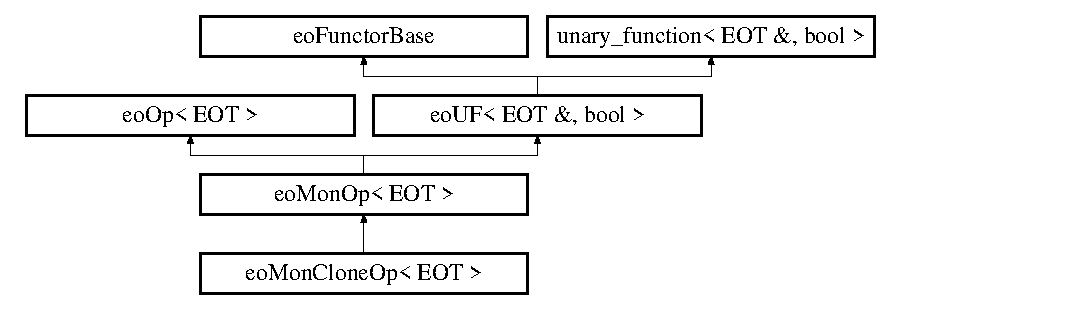
\includegraphics[height=3.71476cm]{classeo_mon_clone_op}
\end{center}
\end{figure}
\subsection*{Public Member Functions}
\begin{CompactItemize}
\item 
{\bf eo\-Mon\-Clone\-Op} ()\label{classeo_mon_clone_op_a0}

\begin{CompactList}\small\item\em Ctor. \item\end{CompactList}\item 
virtual std::string {\bf class\-Name} () const \label{classeo_mon_clone_op_a1}

\item 
virtual bool {\bf operator()} ({\bf EOT} \&)\label{classeo_mon_clone_op_a2}

\begin{CompactList}\small\item\em The pure virtual function that needs to be implemented by the subclass. \item\end{CompactList}\end{CompactItemize}


\subsection{Detailed Description}
\subsubsection*{template$<$class EOT$>$ class eo\-Mon\-Clone\-Op$<$ EOT $>$}

Mon clone: one argument. 



Definition at line 44 of file eo\-Clone\-Ops.h.

The documentation for this class was generated from the following file:\begin{CompactItemize}
\item 
eo\-Clone\-Ops.h\end{CompactItemize}
